
\documentclass[lnicst]{svmultln}
\renewcommand{\arraystretch}{1.5}
\usepackage{amssymb}
\setcounter{tocdepth}{3}

\usepackage{epsfig}
\usepackage{cite}
\usepackage{verbatim}
\usepackage{graphicx}
\usepackage{caption}
\usepackage{subcaption}

\usepackage{url}
\urldef{\mailsa}\path|{collins, rajive}@cs.ucla.edu|
\usepackage[pdfpagelabels,hypertexnames=false,breaklinks=true,bookmarksopen=true,bookmarksopenlevel=2]{hyperref}

\begin{document}

\mainmatter  % start of an individual contribution

% first the title is needed
\title{MELON: A Persistent Message-Based Communication Paradigm for MANETs}

\titlerunning{MELON Communication Paradigm for MANETs}

\author{Justin Collins\and Rajive Bagrodia}
\authorrunning{MELON Communication Paradigm for MANETs}
% (feature abused for this document to repeat the title also on left hand pages)

% the affiliations are given next
\institute{University of California, Los Angeles\\
Los Angeles, CA\\
\mailsa }

\toctitle{MELON: A Persistent Message-Based Communication Paradigm for MANETs}
\tocauthor{Justin Collins and Rajive Bagrodia}


\maketitle
\begin{abstract}
In this paper we introduce MELON, a new communication paradigm tailored to mobile ad hoc networks based on novel interactions with a distributed shared message store. MELON provides read-only messages, per-process tracking of read messages, private messages, and bulk message operations, while addressing the dynamic environment of MANETs. We quantitatively compare a prototype implementation of MELON to existing paradigms to show its feasibility as the basis for new MANET applications. Experiments demonstrate 40\% better throughput on average than traditional paradigms, as well as 70\% faster local insertion and removal operations compared to an existing tuple space library.
\end{abstract}

\section{Introduction}

While smartphones are quickly becoming ubiquitous, most mobile applications continue to use a client-server model instead of communicating through mobile ad hoc networks (MANET). One reason may be the added challenges of developing a MANET application which must communicate with peers over unreliable shifting network topologies. While communicating over a single-hop wireless network (either a WiFi access point or cellular tower) to a central server is simpler, MANETs are useful when communication is between nearby devices (avoiding data charges, for example) or when there is no network infrastructure, such as in disaster recovery situations. Even less dramatic circumstances such as locations without cellular signals can also benefit from MANETs.

To alleviate some of the application development challenges posed by MANETs, several approaches to middleware and libraries have been proposed. The majority of these proposals are based on traditional distributed computing paradigms: publish/subscribe\cite{psfaces}, remote procedure calls\cite{rpc}, and tuple spaces\cite{linda}. In this paper, we introduce a new paradigm called MELON\footnote{Message Exchange Language Over the Network}. MELON provides new communication primitives designed to address the specific aspects of MANETs which make application development difficult, including the most prominent feature of MANETs: frequent network disconnections.

We demonstrate that our proposed paradigm is feasible by comparing performance of MELON to canonical implementations of existing paradigms. On average, MELON had 16\% lower message latency and 71\% higher throughput than tuple spaces. MELON performed with the highest throughput in our experiments, averaging 16\% more messages per second than publish/subscribe, the next fastest paradigm.

The rest of this paper is organized as follows: Section \ref{sec:challenges} lists the MANET challenges we address; Section \ref{sec:design} discusses the design and operations of MELON; Section \ref{sec:implementation} provides details of the MELON implementation; in Section \ref{sec:evaluation} we quantitatively compare MELON to existing paradigms; Section \ref{sec:relatedwork} references related work; and finally Section \ref{sec:conclusion} presents our conclusions.

\section{MANET Application Challenges}\label{sec:challenges}

Applications which are developed for MANETs must operate in an infrastructureless, unreliable, and dynamic distributed environment. This presents a particular combination of challenges which should be addressed by a development platform. In \cite{mine} we identify disconnection handling, addressing and discovery, and flexible communication as important features for MANET development.

Wireless communication can be disrupted in many ways, including competing broadcasts, physical obstacles, and nodal mobility. When combined with an entirely self-organizing network where nodes may join and leave the network at any time, this environment leads to frequent communication disruptions. In traditional networking libraries, disconnections are treated as exceptional events which must be handled by the application. In MANETs, disconnections are so common they should be handled naturally by the programming paradigm.

The dynamicity of MANETs also leads to transience of resources. It is common in distributed programming paradigms to refer to resources independently from the physical location of the resources. This also works well in MANETs, since a resource is likely to be mobile, and several hosts may offer the same type of resource over time.

Before addressing resources an application must discover the resources which are available. The infrastructureless nature of MANETs precludes the use of centralized architectures to maintain a directory of resources. It is also unlikely the location of resources will be known prior to joining a network. Distributed discovery mechanisms are needed to find resources in a MANET environment.

As the primary purpose of a programming paradigm for MANETs is communication between hosts, a general-purpose paradigm should provide flexible communication: both multicast and unicast communication are common in MANET applications. Given the ubiquity of SMS, instant messaging, and direct messages, the paradigm should also support private unicast communication.

Besides the desired features for application development discussed above, it should also be noted that devices in MANETs are often resource constrained. Smartphones have become essentially ubiquitous in many countries and have much less power, CPU, memory, and storage space than a typical consumer desktop computer. These constraints influence the design of paradigms intended for these devices.

\section{MELON Design}\label{sec:design}

The design of MELON is centered around a distributed shared message store. Each device in the network may host any number of applications which access and contribute to the shared message store. Each application hosts a local message store which may be accessed by any other local or remote application. Applications request messages (which may be stored locally or remotely) using message templates.

By communicating through a shared message store, the concept of a connection between hosts is eliminated and thus disconnections are no longer an issue at the application layer. A host suddenly leaving the network does not disrupt an application and applications do not need to handle a communication operation returning an error or failing due to intermittent network connectivity or physical wireless interference. The application is effectively insulated from these issues by the nature of the paradigm and the semantics of the operations.

Messages are sent and received asynchronously by storing and retrieving them from the shared message store, removing the need for a persistent connection. This provides temporal decoupling between hosts, since messages can still be delivered even after prolonged disconnections.

Due to the dynamic network topology of MANETs, maintaining any type of logical or overlay network structure becomes challenging, so MELON does not rely on a particular network structure. Discovery of available messages is performed dynamically for each operation. While this does increase the amount of communication required for each operation, it removes the need for global state and allows the network to change at any time.

MELON also provides spatial decoupling by matching messages based on content, instead of a host address or location. The messages themselves may physically reside on any host in the network. The sender of a message is not aware of the receivers' identities nor even how many receivers might read a message. This frees applications from tracking remote addresses or contacting a directory service to find remote resources.

The shared wireless communication medium in MANETs is well-suited to group or multicast communications. MELON supports multicast communication by allowing any number of receivers to read the same message. MELON also provides bulk receives, which allow applications to efficiently receive multiple messages from multiple hosts in a single operation.

Applications often also require unicast communication. While unicast communication can be accomplished through by storing regular messages in MELON, these can be disrupted by a process removing a message intended for a different receiver. It is also possible to eavesdrop on messages by reading but not removing a message. For applications such as instant messaging, it is important to have private unicast communication. In MELON, messages may be directed to a specific receiver to ensure the messages are only taken by the intended recipient.

MELON also includes features uncommon to shared message stores to further simplify application development in MANETs. First, messages are returned in first-in first-out order per host. When a host receives a message request, it returns the oldest matching message in its local storage. In applications where a single host generates the majority of the messages, this eliminates the need to order messages on the receiver side. 

Secondly, MELON provides operations to only read messages which were not previously read by the same process. This enables an application to read all matching messages currently in the message store, then read only newly-added messages in subsequent operations. It also prevents an application from reading the same message twice.

Finally, MELON differentiates between messages which are meant to persist and be read by many receivers versus messages intended to be removed from the message store. For example, messages in a news feed would have many readers, but the messages themselves should not be removed. On the other hand, a job queue expects each job to be removed by exactly one worker. MELON provides operations to support both of these scenarios.

\subsection{MELON Operations Overview}

Messages can be copied to the shared message store via a \textbf{store} or \textbf{write} operation. A \textbf{store} operation allows the message to later be removed from the storage space. Messages saved with a \textbf{write} operation cannot be explicitly removed from the storage space, only copied.

Messages added via \textbf{store} may be retrieved by a \textbf{take} operation using a message template which specifies the content of the message to be returned. A \textbf{take} operation will remove a message with matching content from the message store and return it to the requesting process. \textbf{take} operations are atomic: a message may only ever be returned by a single \textbf{take} operation.

A \textbf{read} operation will also return a message matching a given template, but does not remove the original message from the shared storage. Any number of processes may read the same message. However, repeated applications of a \textbf{read} operation in the same process will never return the same message. Only messages stored with \textbf{write} can be returned by a \textbf{read} operation.

The basic \textbf{take} and \textbf{read} operations return a single message per invocation. To facilitate the exchange of multiple messages, MELON includes the bulk operations \textbf{take\_all} and \textbf{read\_all}. The bulk versions operate the same as the basic operations, except all available matching messages will be returned instead of a single message. For \textbf{read\_all}, only messages which were not previously returned by a \textbf{read} or \textbf{read\_all} in the same process will be returned.

By default \textbf{take}, \textbf{take\_all}, \textbf{read}, and \textbf{read\_all} will block the process until a matching message is available. MELON also provides non-blocking versions of these operations. The non-blocking operations will return a null value if no matching messages can be found.

When a message is saved with a \textbf{store} operation, it may optionally be directed to a specific receiver. In a directed message, the identity of a receiver is included in the message as the addressee. Only the addressee may access a directed message through a \textbf{take}.

Due to the limited resources of most devices in a mobile network, storage space in MELON is explicitly bounded. Any message may be garbage collected prior to being removed by a \textbf{take} if capacity is reached.

\subsection{Operation Details}

Processes in MELON communicate by storing messages to a distributed shared message store and retrieving the messages based on templates. In this paper, we assume messages consist of an ordered list of typed values and optionally an addressee. However, nothing in the paradigm itself limits how messages might be constructed (e.g., they could be an unordered tuple with named values instead).

A message template is similar to a message, except it may contain both values and types. For example, a message containing \texttt{[1, "hello"]} could be matched by a template containing \texttt{[1, String]} or \texttt{[Integer, "hello"]} or \texttt{[Integer, String]}. A type will also match any subtypes.

Each operation is implemented as a separate function call. \textbf{store} and \textbf{write} operations have null return values and return as soon as the saved message is available in the message store. \textbf{take} and \textbf{read} operations block by default until a matching message is returned, but may be set to non-blocking on a per-call basis.

\begin{table}
\centering
\begin{tabular}{|c|c|c|}
\hline
\textbf{Operation} & \textbf{Return Type} & \textbf{Action} \\ \hline
\textbf{store}(\textit{message}, \textit{[address]}) & \textit{null} & Store removable message \\ \hline
\textbf{write}(\textit{message}) & \textit{null} & Store read-only message \\ \hline
\textbf{take}(\textit{template}, \textit{[block = true]}) & \textit{message} or \textit{null} & Remove and return message \\ \hline
\textbf{read}(\textit{template}, \textit{[block = true]}) & \textit{message} or \textit{null} & Copy and return read-only message \\ \hline
\textbf{take\_all}(\textit{template}, \textit{[block = true]}) & \textit{array} & Bulk remove messages \\ \hline
\textbf{read\_all}(\textit{template}, \textit{[block = true]}) & \textit{array} & Bulk copy read-only messages \\ \hline
\end{tabular}
\caption{MELON Operations}
\end{table}

When called, \textbf{store} saves a copy of the message in the message store. Messages saved with \textbf{store} may only be retrieved with a \textbf{take} or \textbf{take\_all} operation. If an address is provided, then only the host with a matching identity can remove the message.

The \textbf{write} operation also stores a single message in the message store, but the message may only be copied from the storage space with a \textbf{read} operation, never explicitly removed. Messages written with the \textbf{write} operation may be automatically garbage collected.

A \textbf{take} operation requires a message template as the first argument and an optional boolean for the second argument. The message template is matched against available messages in the message store which were added with a \textbf{store} operation. If a matching message is found, it will be removed from the message store and returned. Once a message has been returned by a \textbf{take} operation, it is removed from the message store and may not be returned by a subsequent operation in any process.

The \textbf{read} operation will only return messages stored with a \textbf{write} operation which have not already been read by the current process. If a message matching the given message template is available, it will be copied and returned, but not removed from the message store. Once a message has been returned to a process, the message is considered to have been read by that process and will not be returned by any subsequent \textbf{read} or \textbf{read\_all} operations in that process. A message may be \textbf{read} by any number of processes, but only once per process.

\begin{table}
\centering
\caption{Read from multiple processes}
\begin{tabular}{|c|c|c|} \hline
\textbf{Process A} & \textbf{Process B} & \textbf{Process C} \\ \hline
\texttt{write([1, "hello"])} & \texttt{m = read([Integer, String])} & \texttt{m = read([Integer, String])} \\ \hline
\end{tabular}
\label{fig:readprocesses}
\end{table}

Table \ref{fig:readprocesses} illustrates one process writing a single message containing the integer \texttt{1} and the string \texttt{"hello"}. Processes B and C each perform a \textbf{read} operation with the template \texttt{[Integer, String]} which matches the message stored by process A. Since \textbf{read} does not modify the storage space, the value of \textit{m} for both process B and C will be a copy of the message \texttt{[1, "hello"]} from Process A.

The \textbf{take\_all} and \textbf{read\_all} operations are used to retrieve a group of matching messages instead of a single message. Otherwise, the semantics match \textbf{take} and \textbf{read}: \textbf{take\_all} can only remove messages from \textbf{store} operations, and \textbf{read\_all} only returns unread messages from \textbf{write} operations.

\begin{table}
\centering
\caption{News server and reader}
\begin{tabular}{|c|c|} \hline
\textbf{News Server} & \textbf{News Reader} \\ \hline
\begin{minipage}{2.45in}
\begin{verbatim}

function report(category, headline) {
   write([category, headline])
} 
\end{verbatim}
\end{minipage}
&
\begin{minipage}{2.5in}
\begin{verbatim}


function fetch(category) {
   return read_all([category, String])
}
\end{verbatim}
\end{minipage}
\\ \hline
\end{tabular}
\label{fig:newsreader}
\end{table}

Table \ref{fig:newsreader} demonstrates a use of \textbf{read\_all}. In this example, one or more processes generate news messages containing a news category and headline. To ensure all interested parties can read the news, the server uses \textbf{write} to disallow a reader from removing a news item and preventing other readers from reading it. Any number of processes can consume the news as readers. The \texttt{fetch} method in Table \ref{fig:readprocesses} uses \textbf{read\_all} to return all news items in a given category. Repeated calls to \texttt{fetch} will only return news items not previously seen.

By default, all retrieval operations will block the application until at least one matching message is found. The operations can also be performed in nonblocking mode, in which case \textbf{take} and \textbf{read} return null when no matching message is found, while \textbf{take\_all} and \textbf{read\_all} return empty collections.
   
\section{MELON Implementation}\label{sec:implementation}

\begin{figure}
\centering
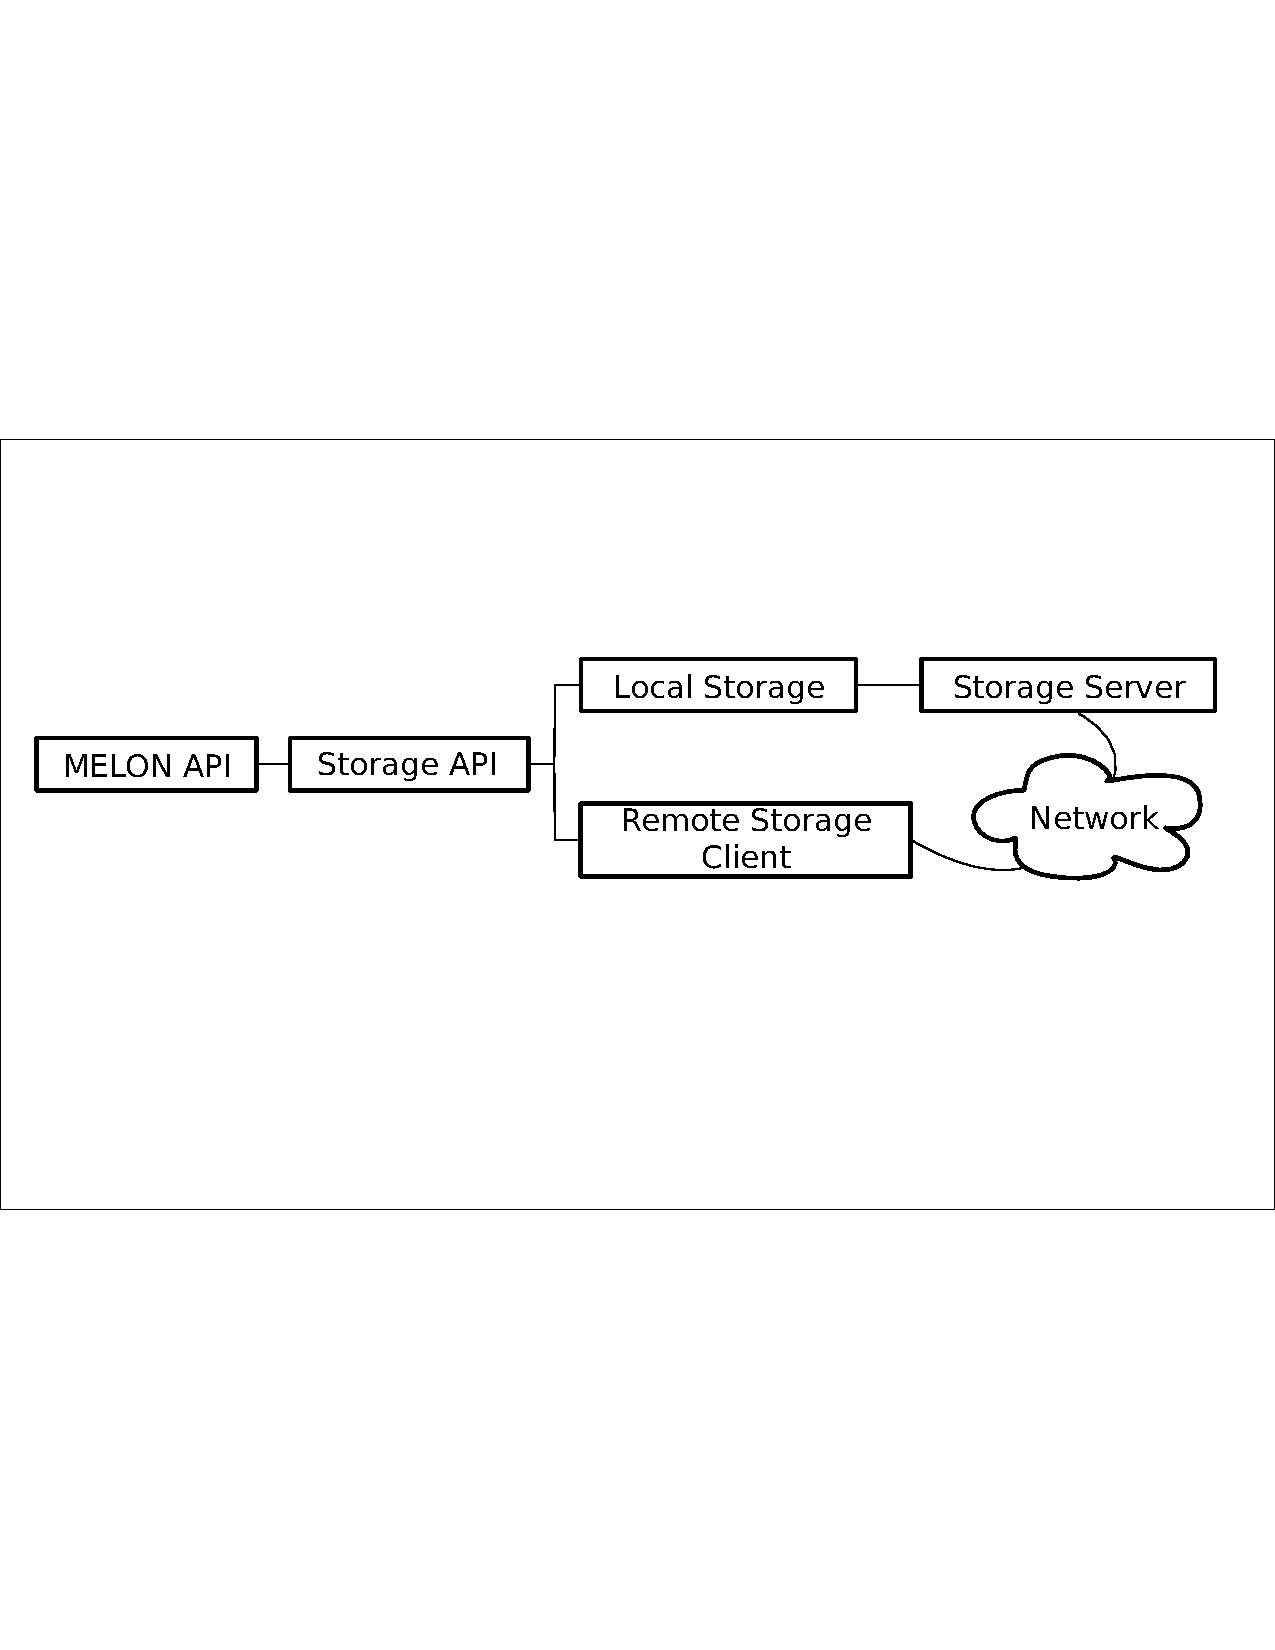
\includegraphics[scale = .50, clip, trim = 10px 350px 10px 312px]{figures/paradigm_arch.pdf}
\caption{Paradigm Architecture}
\label{fig:architecture}
\end{figure}

We developed a prototype implementation of MELON to validate our design and obtain empirical performance data. The architecture illustrated in Figure \ref{fig:architecture} is split into five parts. The MELON API is the only interface exposed to the application and provides the six operations described above. The MELON API interacts with the distributed message storage through the storage API, which provides the same interface for both local and remote storage. The storage server proves a network interface to a local storage space and accepts connections made through the remote storage stub.

Local storage is implemented as two dynamic arrays, one for \textbf{write}/\textbf{read} messages and the other for \textbf{store}/\textbf{take} messages. For atomic updates, the \textbf{write}/\textbf{read} array uses a readers/writer lock to allow multiple \textbf{read} operations to access the array in parallel, but locks the array for \textbf{write} operations. The \textbf{store}/\textbf{take} array does not permit concurrent operations, since both \textbf{store} and \textbf{take} modify the store. The two arrays may be accessed and modified independently.

Network communication is handled using ZeroMQ\cite{hintjens2013zeromq}, a high performance networking library. For the prototype, the networking was intentionally kept simple. For example, a \textbf{read} request queries remote hosts in random order and stops when a matching result is returned. This could possibly be improved using multicast, it would complicate the implementation by requiring the client to handle multiple asynchronous responses, select one, request the actual message, and handle failure scenarios if the matching message cannot be returned. We traded potential performance gains for simplicity. 

For \textbf{read} and \textbf{read\_all} operations, it is necessary to track which messages have been read. Each process maintains its own list of read messages, which it sends with each \textbf{read} request. We use a compact sparse bit set to transfer this information efficiently. We measure this overhead in Section \ref{sec:overhead}.

\section{Quantitative Evaluation}\label{sec:evaluation}

To determine if MELON is a feasible solution for actual MANET applications, we chose to compare its performance to canonical implementations of publish/subscribe, RPC, and tuple spaces. If a prototype implementation of MELON performs at least as well as existing paradigms, then it is likely to be useful in actual practice. In the experiments below, we compare speed of operations, message overhead, throughput, and latency in a MANET context.

\subsection{Experimental Setup}

In order to judge the performance of MELON, we used applications written using the prototype MELON implementation and evaluated them using the EXata network emulator\cite{exata}. Using an emulator allowed us to run real applications but also have precisely repeatable environments with high fidelity network models.

We use a single scenario with 50 nodes distributed in a 150m square grid which move using a random waypoint mobility model. Signal propagation is limited to 50m in order to match an indoor environment and force multihop routes, and the two-ray model is used for path loss. Every run of the mobile scenario uses the same random seed so the mobility pattern is identical. 802.11b WiFi is used with the AODV\cite{aodv} routing protocol.

\subsection{Operation Speed}

\begin{figure}
\centering

\begin{subfigure}{.5\textwidth}
\centering
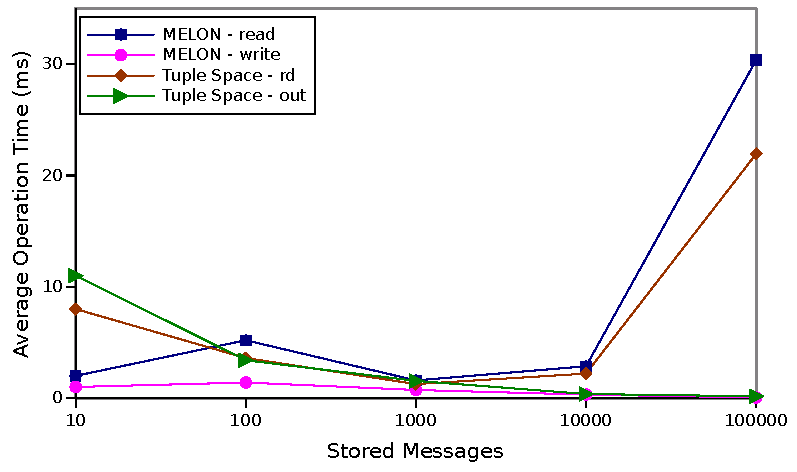
\includegraphics[width = \linewidth, clip, trim = 0px 0px 0px 0px]{figures/read_speed.pdf}
\caption{Read Speed}
\label{fig:readspeed}
\end{subfigure}%
\begin{subfigure}{.5\textwidth}
\centering
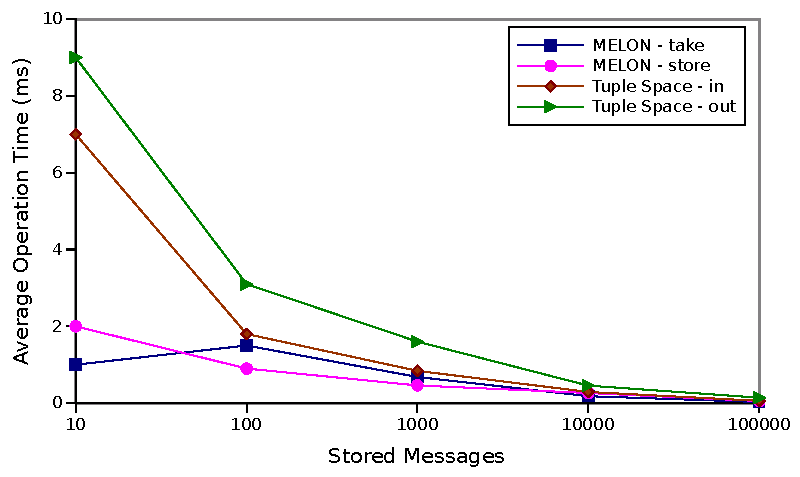
\includegraphics[width = \linewidth, clip, trim = 0px 0px 0px 0px]{figures/in_speed.pdf}
\caption{Take Speed}
\label{fig:takespeed}
\end{subfigure}

\caption{Operation Speeds}
\end{figure}

To establish a baseline for performance, we measured the time for the \textbf{write}, \textbf{read}, \textbf{store}, and \textbf{take} operations directly on a local message storage and compared the results to the LighTS\cite{lights} local tuple space implementation used by LIME. In these experiments, all messages are first stored, then either read or removed from the local storage. No network communication is involved.

When comparing \textbf{read} and \textbf{rd}, we simulate the MELON's feature of only returning unread messages by using a sequential integer ID in the tuples and performing a \textbf{rd} operation for each ID. If we did not do this, LighTS would return the same tuple for each \textbf{rd} operation.

In LighTS and MELON messages are stored in arrays. Operations linearly search the arrays in O(\textit{nm}) time, where \textit{n} is the length of the message and \textit{m} is the number of stored messages. Operations returning messages near the beginning of the array are fastest, while the slowest operation returns the final message. In our experiments, this cost did not become apparent until searching 100,000 messages when average time per operation increased \~9x for LighTS and \~10x for MELON, with total read time taking just under a minute. MELON is slightly slower since it also compares messages to the ``read'' list.

On the other hand, removing messages is fast since the matching message is always the first message in the store. All \textbf{take}/\textbf{in} operations require less than 8\textit{ms} to execute on average. MELON is slightly faster here due to differences in how removal is implemented, although average speed per operation converges as the number of operations performed increases.

Storing messages is naturally faster than removing them for both implementations. In LighTS there is slightly more constant overhead for adding new tuples, so \textbf{out} operations are a little slower than \textbf{write} and \textbf{store} in MELON.  However, in reality both implementations are fast enough for typical applications, since storing a message takes less than 10\textit{ms} on average, and usually less than 4\textit{ms}.

\subsection{Communication Overhead}\label{sec:overhead}

\begin{figure}
\centering
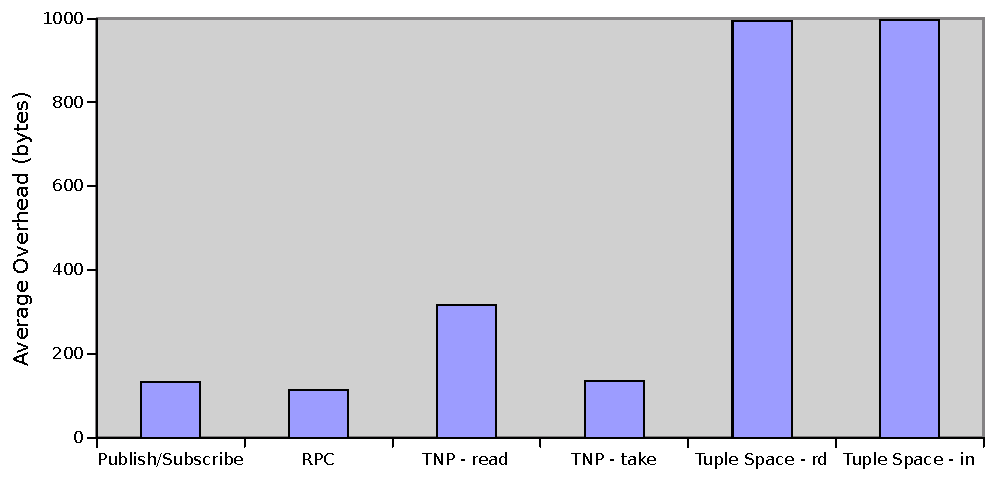
\includegraphics[scale = .50, clip, trim = 0px 0px 0px 0px]{figures/overhead.pdf}
\caption{Message Overhead}
\label{fig:overhead}
\end{figure}

For any communication library or framework, increased message size is an important factor in determining usefulness. We average the number of bytes actually sent over the network per message and subtract the 1KB application payload to determine overhead as shown in Figure \ref{fig:overhead}.

Publish/subscribe and RPC have very low overhead and provide a good baseline. In the case of publish/subscribe, the only added information to a publication is a topic. For RPC, there is one initial exchange to find the remote object, then later messages only need the object and method names plus the payload.

We again use the LighTS tuple space implementation to determine overhead. The serialized versions of tuples and tuple templates are very large and must be sent for each request. If simpler data structures were used, overhead would be expected to be similar to MELON's overhead for \textbf{take}.

For MELON, \textbf{take} and \textbf{read} requests must send a message template, so the size of the request is dependent on how many values the template contains. For \textbf{read} operations, each request must also send information on previously read messages, which increases as the number of read messages increases.

\subsection{Message Latency}

Figure \ref{fig:latency} shows the average operation latency between a client's request for a message and the receipt of the message. In these experiments, a single host writes out 1,000 messages with a 1KB payload, and the other hosts concurrently read the messages. Tuple spaces and MELON used the \textbf{rd}/\textbf{read} operations to retrieve the messages one at a time. As publish/subscribe does not involve a ``request'' beyond the initial operation, latency was measured as the time elapsed between receiving sequential publications.

In these experiments, MELON and tuple spaces were the most affected by the increase in node speed and packet loss, as well as having the highest latency when nodes were at rest. MELON latency increased 29\% and tuple spaces increased 24\%. In contrast, RPC only increased 7\% and publish/subscribe actually had the lowest latency at the highest node speed. Since publish/subscribe is strictly push-based and has very low overhead, it is able to take advantage of the increased opportunities for transferring data that occur when nodes move quickly in a confined space while being less affected by packet loss. On the other hand, MELON and tuple spaces have high overhead and must continually attempt to request messages from remote nodes.

\begin{figure}
\centering

\begin{subfigure}{.41\textwidth}
\centering
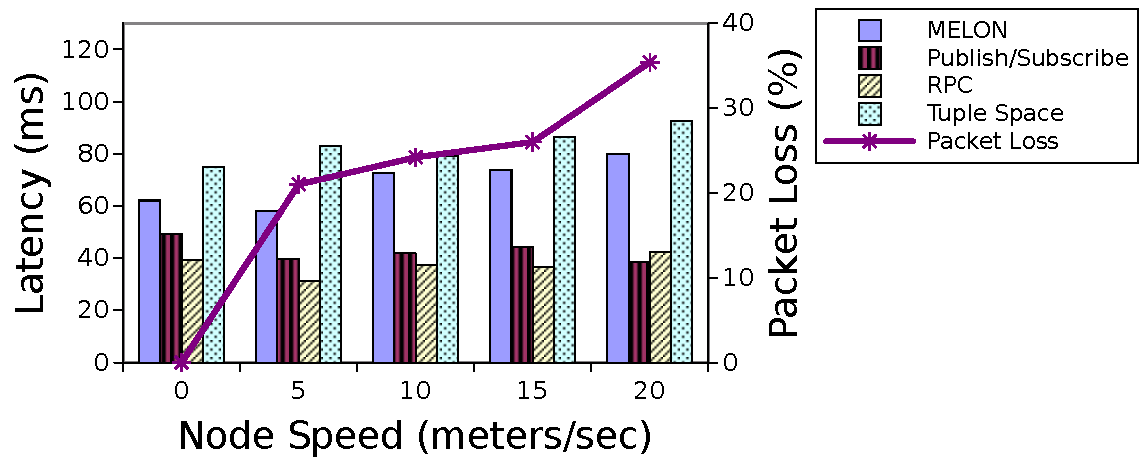
\includegraphics[width = \linewidth, clip, trim = 0px 0px 160px 0px]{figures/latency.pdf}
\caption{Message Latency}
\label{fig:latency}
\end{subfigure}%
\begin{subfigure}{.18\textwidth}
\centering
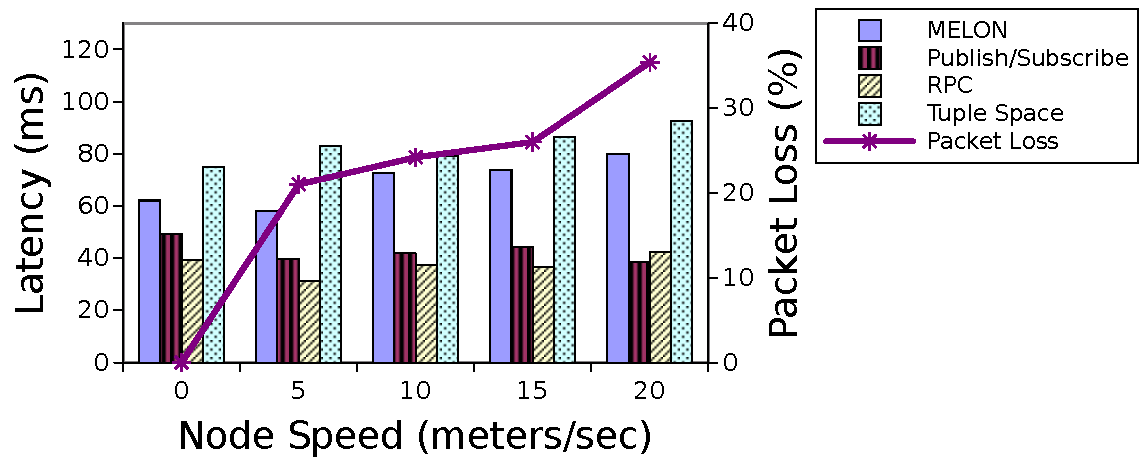
\includegraphics[width = \linewidth, clip, trim = 390px 0px 0px 0px]{figures/latency.pdf}
\end{subfigure}%
\begin{subfigure}{.41\textwidth}
\centering
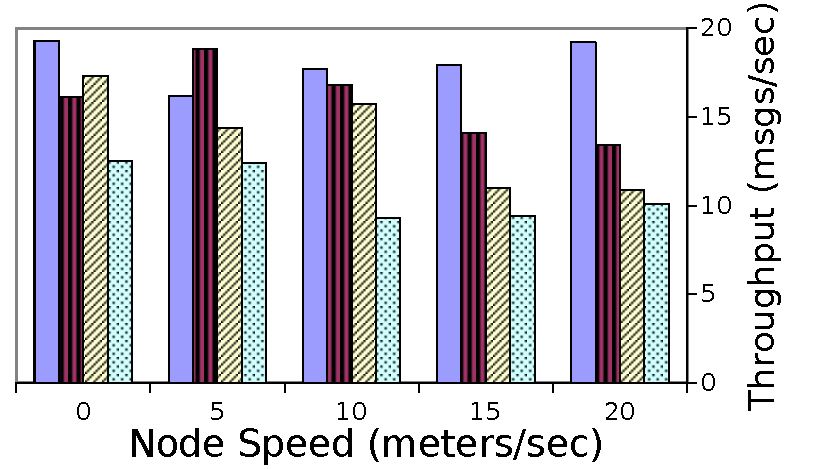
\includegraphics[width = \linewidth, clip, trim = 0px 0px 0px 0px]{figures/throughput.pdf}
\caption{Message Throughput}
\label{fig:throughput}
\end{subfigure}
\caption{Paradigm Performance}
\end{figure}

\subsection{Message Throughput}

Throughput was measured on the receiver side in messages delivered per second. 1,000 messages with a 1kb payload are output by one host, while the other hosts read the messages one at a time. Figure \ref{fig:throughput} shows the average throughput with varying node speeds. Packet loss is identical to Figure \ref{fig:latency}.

Tuple spaces perform the worst, varying from 12.5 to 10.1 messages per second. Given the large overhead, tuple spaces is more affected by packet loss than the other paradigms. MELON provides the best performance in this scenario, delivering between 19.2 and 16.2 messages per second. Both tuple spaces and MELON actually improve slightly as node speed increases from 5 to 20 meters per second. Although higher node speed causes more disconnections between nodes, it also increases the likelihood nodes will be near each other during the experiment.

Publish/subscribe performs well at moderate speeds (18.8 msgs/s at 5 m/s), but since lost messages are lost forever packet loss reduces the number of delivered messages during the experiment, dropping down 29\% to 13.4 msgs/s at 5 m/s.

\section{Related Work}\label{sec:relatedwork}

The concept of a distributed shared message store is based on the idea of tuple spaces introduced with the Linda\cite{linda} coordination language. Several projects have adapted tuple spaces to MANETs, including LIME\cite{lime}, MESHmdl\cite{meshmdl}, TOTA\cite{tota}, and EgoSpaces\cite{egospaces}.

The original version of LIME relies on explicit join and leave operations to federate distributed tuple spaces, which is at odds with the frequently unexpected disconnections in MANETs. \cite{limerevisted} discusses the difficulties LIME encounters when attempting to implement tuple space semantics, including situations that can lead to livelocks. LIME II\cite{lime2}, Limone\cite{limone}, and CoreLIME\cite{corelime} are projects intended to address the shortcomings in the original LIME.

Further surveys of middleware, languages, and communication paradigms for MANET development can be found in \cite{mine} and \cite{mwtrends}.

\section{Conclusion}\label{sec:conclusion}

MELON is a new communication paradigm designed for MANET application and middleware development. It provides a unique combination of new features for interacting with a distributed shared message store, including separation between read-only messages and removable messages, private messages, bulk message operations, and tracking of read messages. In this paper we used real applications to compare MELON performance to existing communication paradigms and demonstrated the new paradigm has acceptable overhead and performance in a MANET context, as well as being useful for general purpose applications.

There are several aspects of MELON which can be explored in future work including message replication, garbage collection, and secure communication. Message replication is very useful in MANETs to overcome network partitioning and increase availability. On the other side, garbage collection of old (and replicated) messages is necessary to keep the MELON storage requirements low for small devices. While MELON does offer direct communication, encrypting private communications is necessary for full security against eavesdropping.

\bibliographystyle{unsrt}
\bibliography{refs}

\end{document}
